\documentclass[12pt]{article} % Default font size of the document, change to 10pt to fit more text

\usepackage{newcent} % Default font is the New Century Schoolbook PostScript font 
%\usepackage{helvet} % Uncomment this (while commenting the above line) to use the Helvetica font

\usepackage[utf8]{inputenc}
\usepackage[francais]{babel}
\usepackage[T1]{fontenc}

% Graphics preamble
\usepackage{graphicx} % Allows to import images
\usepackage{float} % Allows for control of float positions

\usepackage[margin=1.4in,includefoot]{geometry}

\begin{document}

\begin{titlepage}
	\begin{center}
	\line(1,0){400} \\
	[0.25in]
	\huge{\bfseries Analyse d'un Carrefour} \\
	[2mm]
	\line(1,0){300} \\
	[1.5cm]
	\textsc{\LARGE UV 5.8 Ingénierie Systèmes} \\
	[0.75cm]
	\textsc{\Large Bureau d'études – Simulation} \\
	[10cm]
	\end{center}
	\begin{flushright}
	\textsc{\large Evandro Bernanrdes \\ Mohammed Shéhade \\ Sergio Pertierre do Monte  \\}
	\end{flushright}

\end{titlepage}

% Table of contents
\tableofcontents
\thispagestyle{empty}
\cleardoublepage


% List of figures, list of tables
\listoffigures
\cleardoublepage

\setcounter{page}{1}

\section{Objectif de l'étude}\label{sec:1}
La présente étude a comme but trouver une solution qui améliore le trafic d'un quartier de la ville de Brest qui pâtit des embouteillages.

\begin{figure}[H]
	\centering
	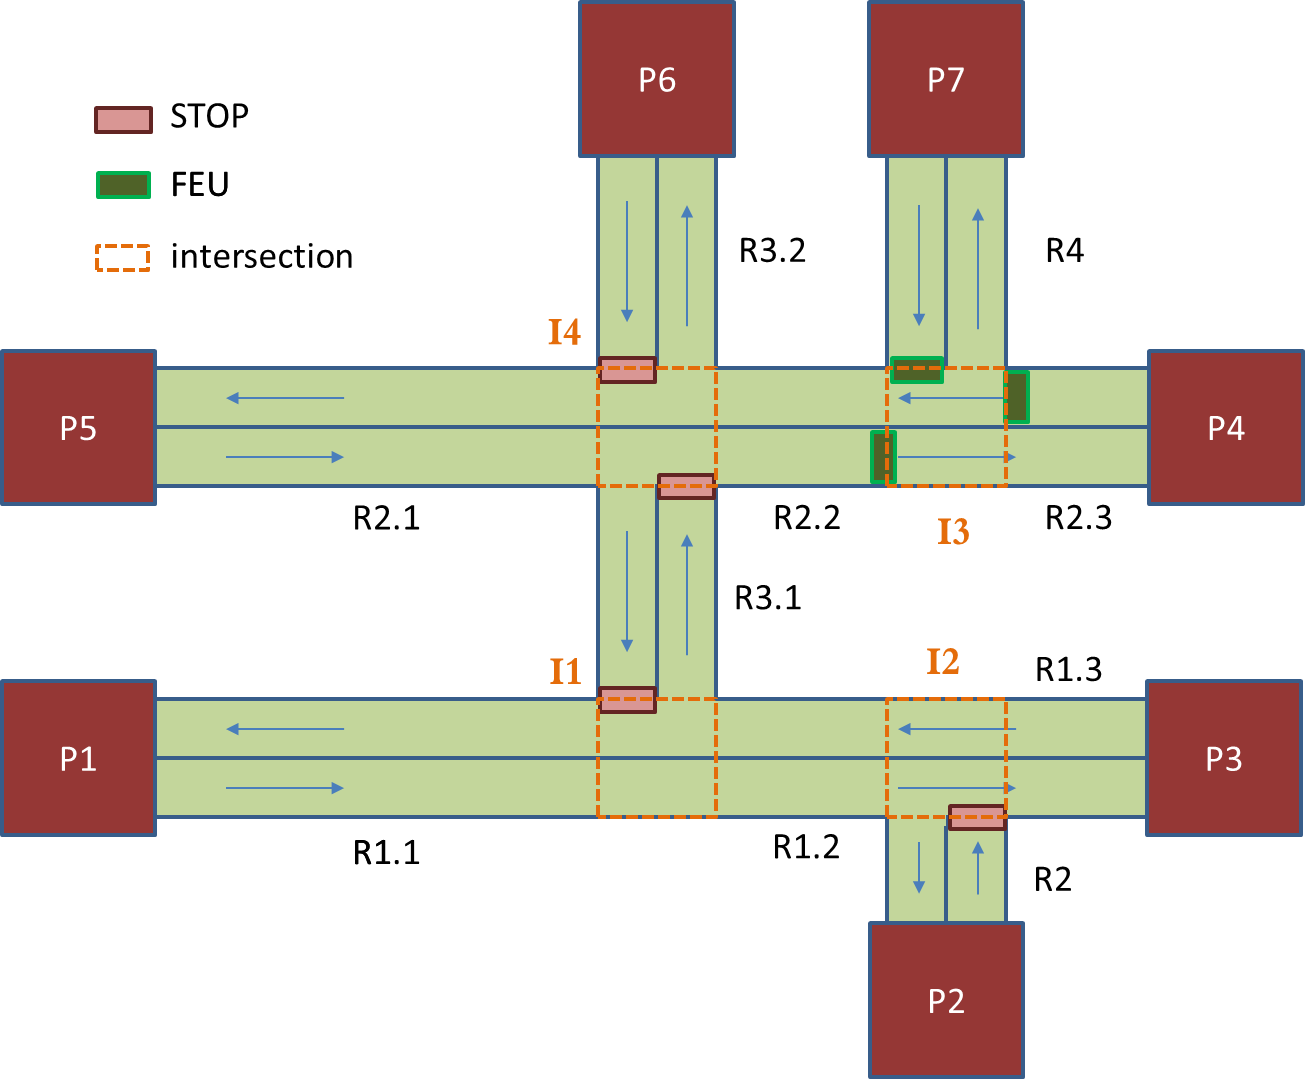
\includegraphics[height=3in]{Figure1.png}
	\caption[Figure 1]{Carrefour Routier de Coruscant}
	\label{fig:fig1}
\end{figure}

Le maire de Brest, M Remai, souhaite améliorer le trafic dans le grand carrefour routier « Coruscant » suite à plusieurs plaintes apportées par les usagers de ce quartier à cause de nombreux embouteillages. Donc, M Remai a demandé à la société TrafBreizh de faire une étude de l'évolution du quartier pour y trouver des solutions.

D’ailleurs, étant donné que cette situation existe en autres zones, le maire a mis plusieurs tranches optionnelles dépendant de la réussite de cette première tranche.

L'entreprise TrafBreizh a comme objectif développer un outil efficace qui puisse résoudre le problème et qui soit capable de s'adapter à d'autres problèmes futures.

Donc, d'abord, pour trouver la solution de cette tâche, en utilisant un moteur de simulation on cherche recréer l'environnent du quartier avec les données fournies qui montrent les caractéristiques des différentes parties élémentaires pertinentes à l'analyse du problème, telles comme les zones d'accès au carrefour et ses routes, l'accélération et la longueur des véhicules, le fonctionnement des feux.

Aussi, pour faciliter cette simulation on a adopté quelques hypothèses pour les voitures comme sera montré ultérieurement, par exemple, elles ont la même taille et suivent les lois de circulation française.

Donc, après avoir obtenu les résultats, on a changé plusieurs paramètres de la simulation en utilisant les exigences du client pour obtenir une solution optimale.
\newpage
\section{Analyse du problème}\label{sec:2}
Plusieurs sous-systèmes doivent être implémentés pour l’implémentation de cette simulation. Un système qui crée tout l’environnement au démarrage et qui démarre le moteur de simulation. Aussi un système qui calcule le chemin à être suivi selon les endroits de départ et d’arrivée de chaque voiture, et un système de création de voitures. 

\subsection{Environnement et variables d'état}
L’environnement compte avec plusieurs entités. Les principales sont : 

\begin{itemize}
\item \textbf{Véhicules :}
Une entité modélisant les véhicules. Chaque voiture doit avoir des variables comme : vitesse, lieux de départ et arrivée, position actuelle, route actuelle, une référence qui indique la voiture qui est juste devant et des variables booléens indiquant quelques états : si la voiture est déjà arrivée, si elle est en train d’attendre le feu vert, si elle est bloquée par une voiture qui est devant. 

\item \textbf{Routes :}
Une classe pour modéliser les routes. Elle doit être munie d’une liste des voitures actuellement présentes, des intersections, les endroits de début et de fin, le nom de la route. 

\item \textbf{Intersections :}
Cette classe doit contenir des références vers les routes qu’elle connecte, des références vers les voitures qui attendent sur chaque route connectée. Aussi faut-il créer un système pour bien implémenter le type d’intersection : Combien de routes elle connecte, s’il y a des feux ou pas. 
\end{itemize}

\subsection{Liste des évènements}
En plus, il faut implémenter les événements importants de la simulation : 

\begin{itemize}
\item La création d'un objet véhicule (simulant l'arrivée d'une voiture dans le quartier); 

\item Le passage des feux vert; 

\item Quand il faut qu'une voiture s'arrête pour attendre les feux; 

\item Un événements de mise à jour des entités (routes, voitures, etc...).
\end{itemize}

%\subsection{Hypothèses particulières}

\newpage
\section{Modélisation du système}\label{modelisation}
This is

\newpage
\section{Implémentation du modèle}\label{implementation}
Le logiciel implémente des classes décrites dans quelques paquets de code Java. Les paquets utilisés sont le paquet « core » et le paquet « components », implémentant un système robuste et versatile de simulation qui peut être utilisé pour la création de plusieurs types d’environnement réels.

\subsection{Paquets du moteur de simulation :}
Le cœur du moteur de simulation, implémente (entre autres) les classes suivantes :

\begin{itemize}
\item \textbf{SimEngine :}
La classe SimEngine est la classe principale qui crée le moteur de simulation. Elle dépend de la graine générant les numéros aléatoires, entre autres paramètres.

En plus, dans cette classe il y a un système de notification (un « Listener ») qui notifie tout changement d'état du moteur. 

Après la mise en place du moteur de simulations avec les paramètres desquels il dépend, la simulation doit être lancé en exécutant une méthode d'initialisation, qui traite chaque événement présent dans une liste dynamique d'événements. 

\item \textbf{SimObject :} Cette classe abstraite joue le rôle de l’entité manipulé le moteur de simulation, et doit connaître qui est le moteur de simulation qui doit l'animer.
Un SimObject a un nom et un identifiant unique, et peut être activé ou désactivé.

\item \textbf{SimTimeEvent :} Classe modélisant un événement temporel.

\item \textbf{SimEntity :} Hérite de SimObject, cette entité de simulation apporte de nouveaux services, comme des constructeurs utilisant les paramètres de l’entité, une gestion d’entités filles, et une gestion du cycle de vie de l’entité. Des Listeners permettent de notifier les changements d’état du système.

\end{itemize}

\subsection{Système implémenté}
Le système implémente une classe « Monitor » qui joue le rôle de la méthode principale. Elle initialise deux loggers, un pour la sortie standard qui montre l'état après chaque événement et un autre qui crée un fichier dans lequel les résultats de la simulation seront sauvegardés. Pour le deuxième, le Monitor doit savoir où créer le fichier.

Suivant l'initialisation des loggers, le Monitor initialise le moteur de simulation, dont l'heure initiale et la durée de la simulation sont données comme paramètres. 

La troisième partie est la création de l'environnement. Le logiciel prend un fichier csv qui décrit la simulation, c'est-à-dire, quels intersections auront des feux et quels intersections sont simples. Le fichier possède ces informations en forme d'une variable binaire pour chaque intersection (1 si intersection simple, 2 si intersection avec des feux).
%
Ces paramètres sont utilisés dans le constructeur de la classe CreationEnvironnement, qui crée tous les entités de la simulation : les routes et les intersections (les informations pour la création des routes sont codes dans la classe CreationEnvironnement pour simplicité. Si jamais on veut réutiliser le même code pour un quartier différent, soit les routes/intersections doivent être changées pour décrire le nouvel environnement, soit ces informations doivent être inclues dans le fichier de paramètres (et la méthode doit être capable de lire ces informations, bien évidemment).
%
Cet objet environnement possède trois listes :
\begin{itemize}
\item \textbf{private LinkedList<StartEnd> listeStartEnd} : Pour savoir quels sont les points possibles d'arrivée et départ (objet StartEnd);

\item \textbf{private LinkedList<Intersection> listeInter} : Les intersections;

\item \textbf{private LinkedList<Route> listeRoute} : Pour sauvegarder les routes crées par le constructeur.
\end{itemize}

Pour finir, le Monitor lance la simulation, attend qu'elle finisse et ferme le logger créant le fichier des résultats.

\newpage
\section{Compte-rendu de V\&V}\label{VV}
This is

\newpage
\section{Résultats de la simulation}\label{resultats-sim}
This is

\newpage
\section{Analyse des résultats}\label{resultats-analyse}
This is

\newpage
\section{Perspectives d'évolutions}\label{evolution}
Pour qu’un meilleur logiciel de simulation puisse être implémenté, plusieurs modifications peuvent être envisagées : 

\begin{itemize}
\item Les voitures ne sont pas toutes identiques, c’est-à-dire, des modèles probabilistes peuvent être développées pour les paramètres décrivant les voitures. 

\item La création d’un modèle plus réaliste pour le redémarrage de la voiture. 

\item Trouver une manière de modéliser les événements particuliers (véhicule qui passe devant celui d’avant, par exemple). 

\item Changer la méthode d'initialisation du système pour que les routes/intersections puissent aussi être facilement créées pour simuler d'autres quartiers.

\item Ajouter une option pour étudier comment un accident ou une obstruction sur une de routes peut impacter les autres.
\end{itemize}




\end{document}